
\section{Introduction}
\label{sec:Introduction}
%%%%%%%%%%%%%%%%%%%%% Vision %%%%%%%%%%%%%%%%%%%%%%%%%
%The goal of this work is to provide power, control, and planning for planar manipulation with soft robots using fluidic elastomer actuators.
The goal of this work is to provide and compare multiple actuator morphologies and multiple fabrication processes for planar soft fluidic elastomer robots.
%
We experimentally validate these morphologies and processes in the context of extremely soft and highly compliant robotic manipulators shown in Figure~\ref{fig:intro}.
%
These manipulators are design to integrate into an autonomous planar manipulation system whose power, control, and planning subsystems are detailed in [CITE].

Soft robots exhibit continuum body motion, large scale deformation, and relatively high compliance compared to traditional rigid-bodied robots \citep{trivedi2008soft}.
%
Such characteristics give this class of robots advantages like the ability to mitigate uncertainty with passive compliance \citep{mcmahan2006field}, perform highly dexterous tasks \citep{deimel2014novel}, and exhibit resiliency \citep{tolley2014resilient}.
%
This work uses softness to develop an entirely new manipulator morphology: that is, a multi-segment planar manipulator composed from soft elastomer and powered by fluids.

\begin{figure}[ht]
\centering
        \begin{subfigure}[t]{0.7\columnwidth}
        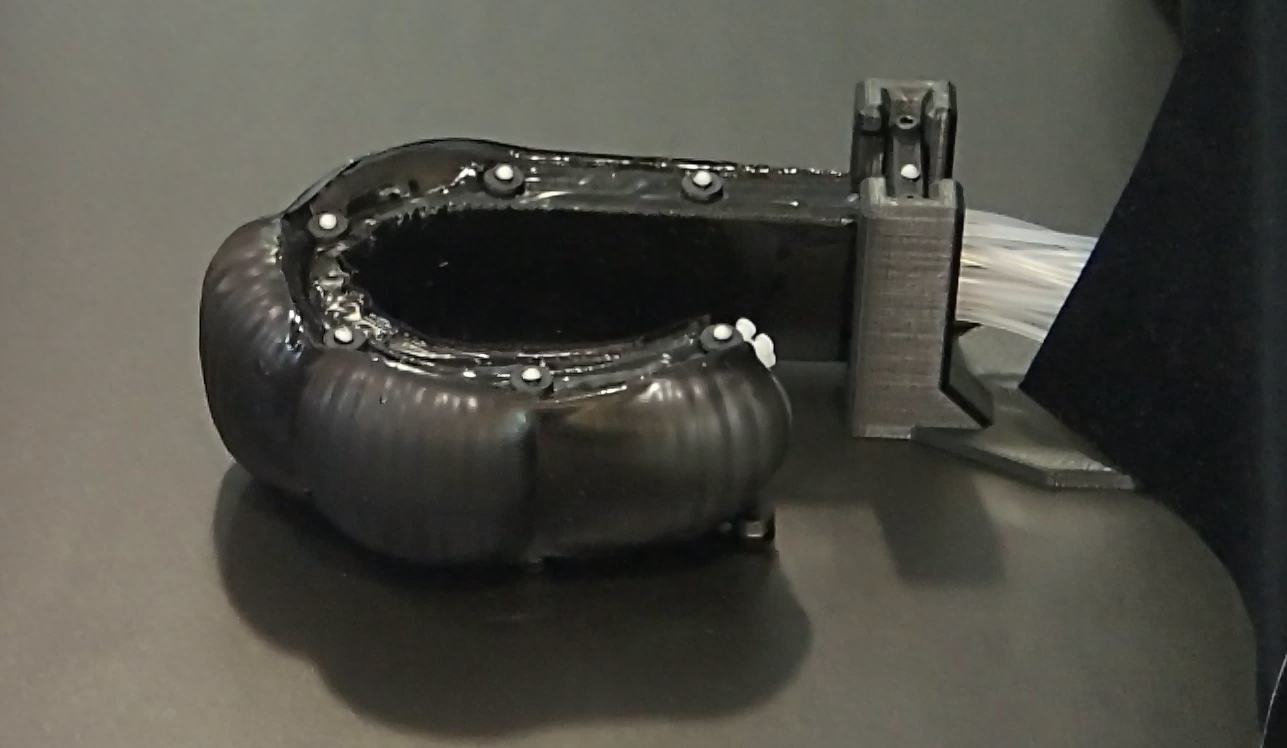
\includegraphics[width=\textwidth]{figures/introduction/ribbed_introduction}
        \end{subfigure}\\
        \begin{subfigure}[t]{0.7\columnwidth}
        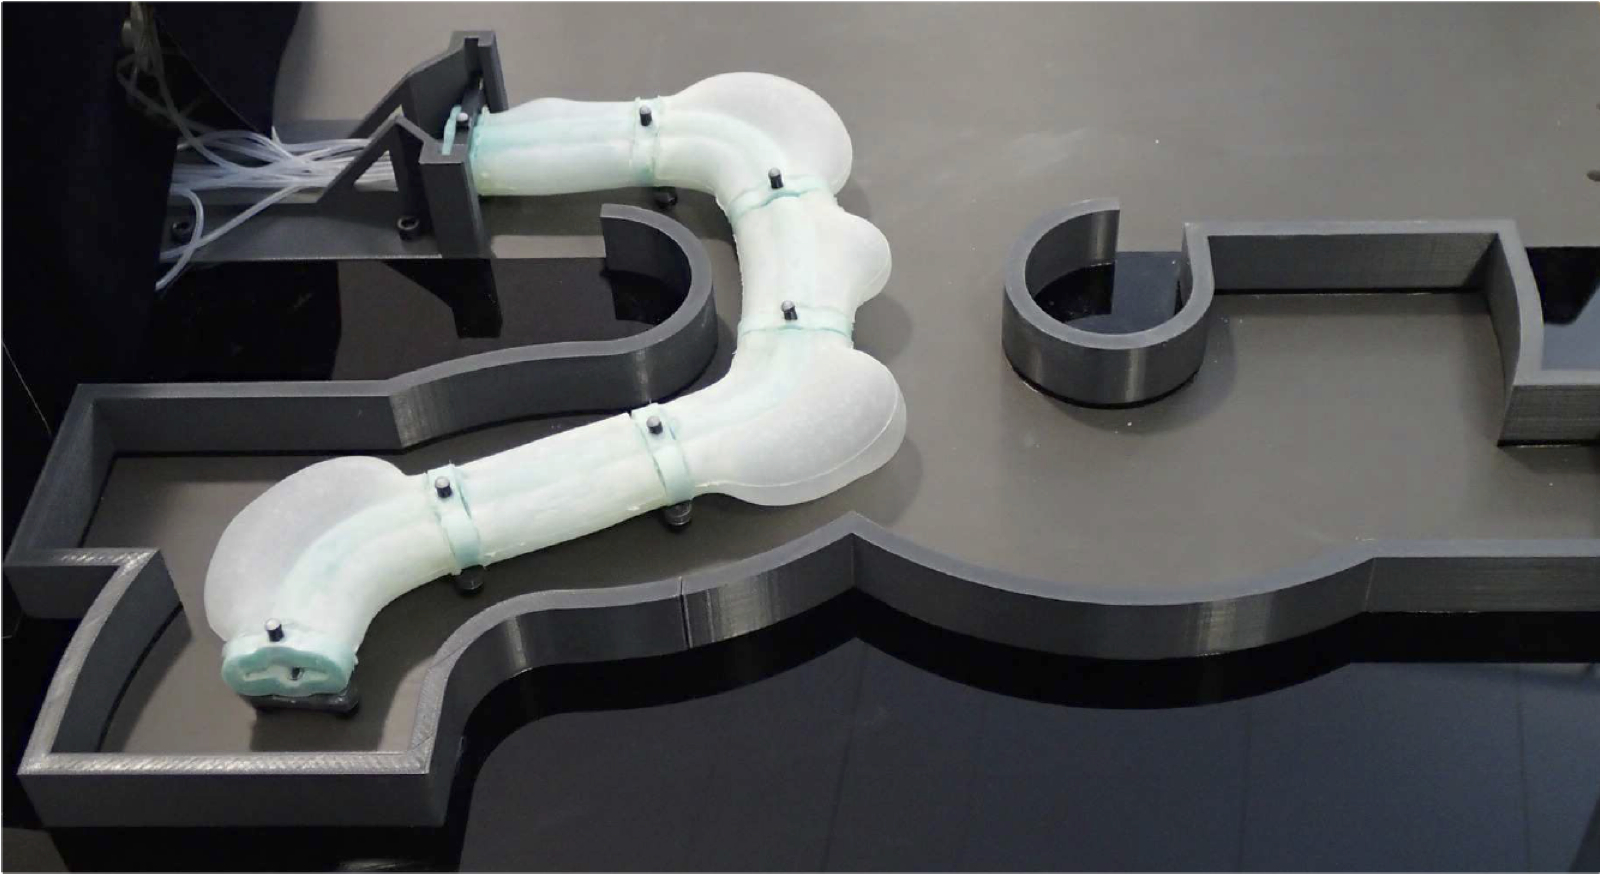
\includegraphics[width=\textwidth]{figures/introduction/cylindrical_introduction}
        \end{subfigure}\\
        \begin{subfigure}[t]{0.7\columnwidth}
        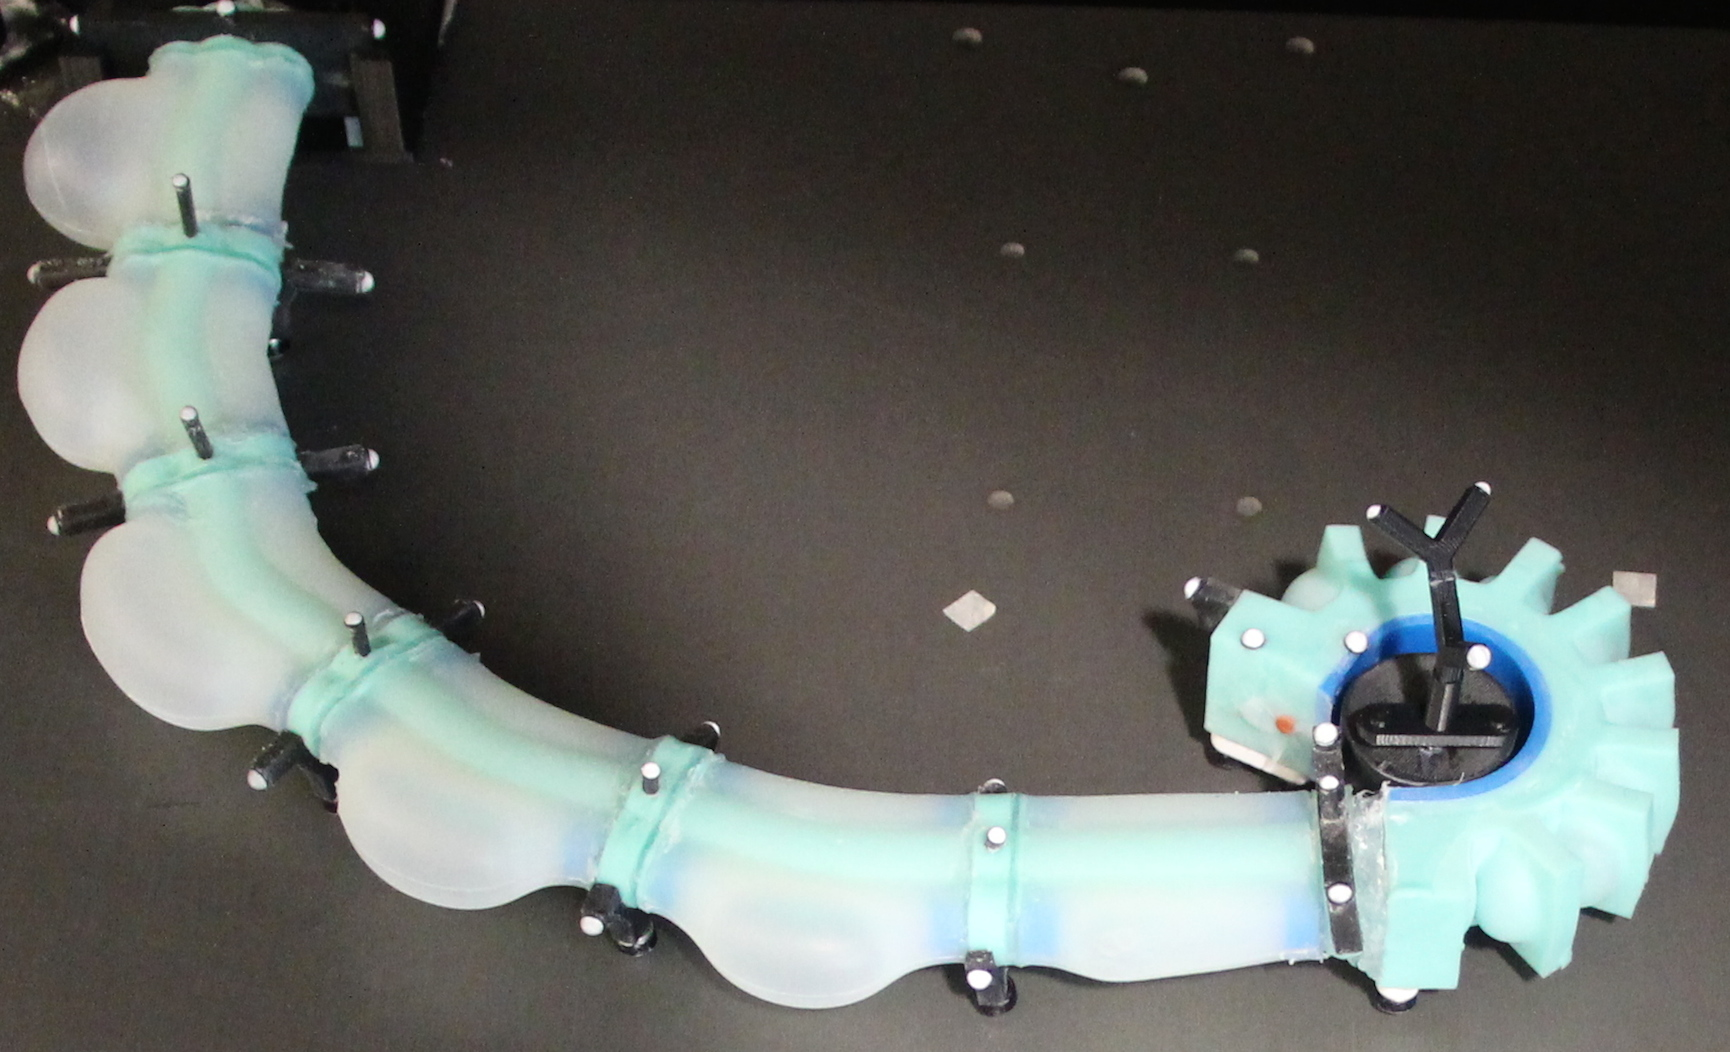
\includegraphics[width=\textwidth]{figures/introduction/gripper_introduction}
        \end{subfigure}
        \caption{Extremely soft and highly compliant robotic manipulators capable of autonomously performing tasks such as point-to-point movements, maneuvering in confined or cluttered spaces, and grasping objects.}
	\label{fig:intro}
\end{figure}


%%%%%%%%%%%%%%%%%%%%% Challenges %%%%%%%%%%%%%%%%%%%%%%%%%
\subsection{Challenges}
Recent reviews \citep{} articulate the challenges associated with creating robots from soft, nonlinear materials.
%
To summaries, current engineering tools are well-suited 
To create fluidic elastomer manipulators, we must overcome many technical challenges, many of which have to do with design and fabrication.
%In general, fluidic elastomer manipulators are highly compliant and their motions are not as precise as more traditional rigid body robots.
More specifically, this work addresses the following challenges:
(i) We do not have a multi-segment fluidic elastomer robot design suitable for automated manipulation.
That is, we need to identify appropriate planar actuator morphologies and ways of assembling these actuators into manipulators.
(ii) Consistently reproducing certain properties of soft robots, for example their elasticity or internal channel geometry, is difficult using conventional fabrication techniques.
Accordingly, we must develop fabrication techniques that balance the competing goals of scalability and repeatability with need of complicated features and shape profiles.
%(i) To the best of our knowledge, there does not exist a closed-loop method for controlling the deformation of fluidic elastomer robots.
%Current robots rely on the concept of morphological control.
%The task of manipulation necessitates the development of new hardware as well as control structures which enable closed-loop configuration control.
%It is difficult to control the soft arm's configuration due to both the compliance of its low-pressure fluidic power system as well as the arm's inherent elasticity.
%(ii) To date, these robots do not have a predictable way of positioning themselves in task space, but this is a fundamental ingredient to manipulation.
%To achieve this, we need to identify appropriate forward and inverse kinematic algorithms for this class of arm.
%As one might expect, the manipulator's inherent compliance complicates the process of modeling and sensing the kinematics.
%(iii) Lastly, planning for fluidic elastomer arms is unexplored. In order to autonomously complete manipulation tasks, we need to develop planning algorithms.

%%%%%%%%%%%%%%%%%%%%% Approach %%%%%%%%%%%%%%%%%%%%%%%%%
\subsection{Approach}
%In this work, we demonstrate that autonomous manipulation with soft fluidic elastomer robots is possible.
First, we present the design and characterization of three fluidic elastomer manipulator morphologies.
Each of the arm's serially connected body segments are fundamentally constructed from derivatives of fluidic elastomer actuators (FEAs) \citep{correll2010soft} and these actuators deform by bending about a neutral axis when pressurized \citep{onal2011soft}.
Next, we provide three alternative fabrication approaches for reliably fabricating these manipulators.
%First, we provide a brief overview of three fluidic elastomer manipulator morphologies.
%Then, a method for closed-loop positional control of these soft manipulators is developed.
%This capability requires two critical innovations.
%First, we solve the previously unaddressed problem of controlling the configuration of an entirely soft and highly compliant pneumatic arm.
%That is, we develop real-time, closed-loop curvature controllers that drive the bending of the manipulator's soft pneumatic body segments despite their high compliance and lack of kinematic constraints.
%Specifically, to achieve curvature control we use an array of cascaded PI and PID controllers as well as develop an array of fluidic drive cylinders to power the manipulators.
%Second, we apply a simplifying piecewise constant curvature (PCC) assumption to model the forward and inverse kinematics relationship between the arm's configuration space, that is the segment curvatures and lengths, and task space, that is cartesian poses of points along its backbone.
%This is done in a manner consistent with traditional continuum manipulation literature, as reviewed by \citet{webster2010design}.
%Under this assumption, we develop forward and inverse kinematics algorithms to transform between configuration and task space.
%
%We combine all these developments into an aggregate system for which we create a suite of planning algorithms, showcasing novel capabilities for this class of robots.
%First, using a Jacobian-based approach to the inverse kinematics problem, we experimentally evaluate the arm's ability to repeatably move to points in free-space as well as track linear end-effector trajectories.
%
%Second, we provide an approach for autonomously moving a planar fluidic elastomer arm through a confined, pipe-like environment.
%We provide a computational approach to whole arm planning that finds a solution to the inverse kinematics problem for this class of arms.
%The solution considers both the primary task of advancing the arm's end effector pose as well as the secondary task of positioning the whole arm's changing envelope in relation to the environment.
%Specifically, we find a transformation from the arm's task space to its configuration space that is aware of the soft arm's entire shape.
%We achieve this by posing a series of constrained nonlinear optimization problems and solving for locally-optimal configuration space parameters.
%A key feature of our approach is that we do not prevent collisions, but rather minimize their likelihood.
%In fact, since we have designed an entirely soft and compliant robot, we can we tolerate collisions.
%Often, the arm's ability to passively comply with the environment allows the primary task to be accomplished despite the collision.
%To experimentally validate the soft robot's ability to successfully advance through a confined environment, we carry
%out a series of experiments using a six segment soft planar manipulator.
%The primary goal of these experiments is to validate the whole body planner's ability to incrementally advance the robot through various pipe-like sections.

%Lastly, we use a fluid-powered gripper for these soft manipulators that can conform to variations in object geometry while ensuring encapsulation of a round object.
%%The gripper is inspired by fingers developed by \citet{polygerinos2013towards} and is advantageous for grasping because it exhibits high curvature, minimal radial expansion, and remains compliant during actuation.
%We attach this gripper to a multi-segment soft manipulator to enable grasp-and-place capabilities.
%We also present a planning algorithm that advances the arm through all necessary states of the grasp-and-place operation.
%The system first plans concentric approach circles shrinking from the initial end-effector pose to the object.
%Next, the system searches for locally-optimal manipulator configurations that constrain the end-effector to lie on these approach circles, so that the manipulator does not collide with the object.
%We experimentally validate the system's ability to repeatably and autonomously grasp-and-place randomly placed objects with a 7 degrees of freedom planar fluidic elastomer manipulator prototype.

%%%%%%%%%%%%%%%%%%%%% Contributions %%%%%%%%%%%%%%%%%%%%%%%%%
\subsection{Contributions}
%The primary contribution of this work is a novel power and computational control and planning system for 2D fluidic elastomer manipulation that enable grasp-and-place and planned continuous motion in environments with obstacles.
%This work is first to show that planar manipulation with soft fluidic elastomer robots is possible and first to provide an approach for closed-loop control and planning of such manipulators.
Specifically this contribution consists of:
\begin{enumerate}
  \item Three viable multi-segment manipulator morphologies that are (i) composed primarily of soft silicone rubber, (ii) powered by fluids, (iii) suitable for automation;
  \item Three fabrication processes for reliably manufacturing these soft fluidic elastomer manipulators;
  %\item The first method for closed-loop configuration control for a soft fluidic elastomer robot consisting of (i) a kinematic model and an algorithm for estimating the manipulator's configuration in real-time, (ii) a novel device for providing continuous, closed-circuit adjustment of the manipulator's fluid, and (iii) a cascaded curvature controller;
%  \item Task-space planning algorithms that solve the IK problem and enable these manipulators to autonomously (i) position their end-effector in free-space, (ii) maneuver in confined environments, and (iii) grasp-and-place objects.
\end{enumerate}
This work is based on three previous conference publications: \citep{marchese2014design}, \citep{marchese2014whole}, and \citep{katzschmann2015autonomous} (in revision). %TODO remove if not in revision anymore 